% TODO
%
% Steckbrief
% History
%

\begin{multicols}{3}[\section{IrDA}]

\rhead{Elias Holzmann, Mirko Grothe}
\lfoot{17.05.2016}

\newrefsegment

\begin{tabular}{p{2,1 cm}p{2.7 cm}}
\textbf{Steckbrief}& \\
\end{tabular}
\rowcolors{1}{\topicolor!20}{}
\begin{tabular}{p{2,1 cm}p{2.7 cm}}
     Einsatz seit & 1993\\
     Wellenlänge  & 850 - 900 nm\\
     Datenrate & 2,4 kbit/s - 10 Gbit/s (noch in Entwicklung) \\
     Einsatzzweck & Datenübertragung von und zu mobilen Geräten \\
\end{tabular}
\par


\subsection*{Überblick}
\begin{wrapfigure}{r}{0.4\linewidth}
  \vspace{-20pt}
  \begin{center}
  	\hspace{-20pt}
    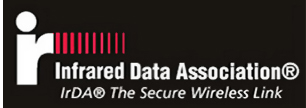
\includegraphics[width=0.7\linewidth]{Kapitel/IrDA/Grafiken/logo_irda.png}
  \end{center}
  \vspace{-15pt}
\end{wrapfigure}
Die \textbf{IrDA} (\textit{\textbf{I}nfra\textbf{r}ed \textbf{D}ata \textbf{A}ssociation}) ist eine 1993 gegründete Vereinigung. Zur damaligen Zeit war Bluetooth noch nicht im Einsatz und die Datenübertragung zwischen PDAs, Notebooks und anderen mobilen Geräten erfolgte über proprietäre Protokolle, meist via \textbf{I}nfra\textbf{r}ot (\textbf{IR}). Die IrDA hatte das Ziel, ein Protokoll zur Datenübertragung zu definieren, das die folgenden Bedingungen erfüllt:
\begin{itemize}
	\item offen, interoperabel
	\item kosteneffizient
	\item angemessen für eine großen Anzahl von Endgeräten~\cite{irdamarketing}
\end{itemize}

Aufgrund des Ziels der Kosteneffizienz wurde IR als Medium gewählt. Hierdurch sind nur eine LED und eine Photodiode notwendig, um einen Transceiver zu fertigen.~\cite{hparticle}

\subsection*{Technische Erläuterungen}
\begin{Figure}
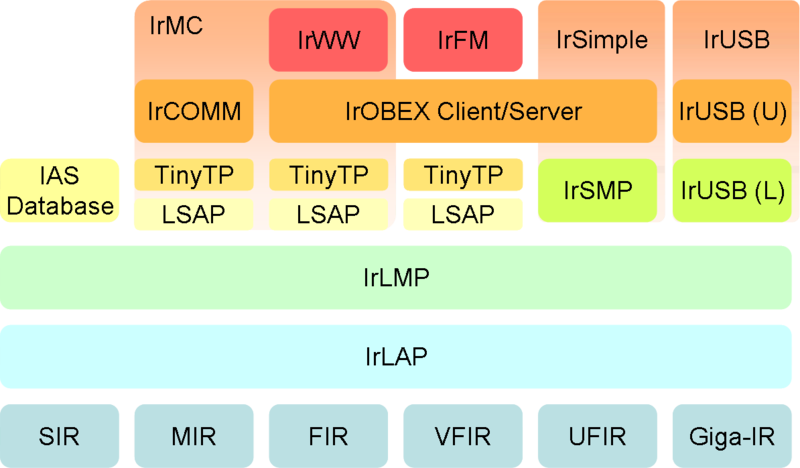
\includegraphics[width=\linewidth]{Kapitel/IrDA/Grafiken/protocol_stack.png}
\captionof{figure}{Übersicht über das IrDA-Protokoll~\cite{wikipediaen}}
\label{fig:irda.stack}
\end{Figure}
Die IrDA hat nicht wirklich ein einzelnes Protokoll spezifiziert, sondern vielmehr eine Protokollfamilie, vergleichbar mit dem TCP/IP-Protokollstack. In den folgenden Abschnitten werden die einzelnen Protokolle näher erläutert.
\subsubsection*{IrPHY}

\begin{Figure}
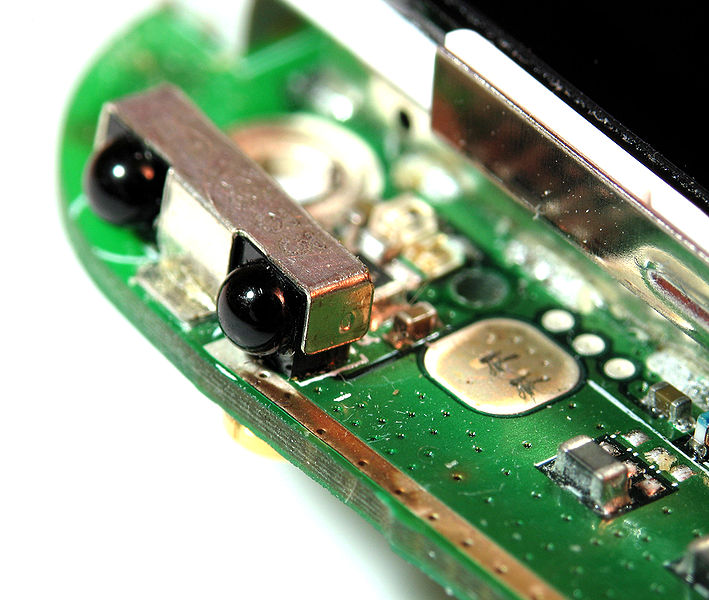
\includegraphics[width=\linewidth]{Kapitel/IrDA/Grafiken/irda_trans.jpg}
\captionof{figure}{Nahaufnahme eines IrDA-Transceivers, bestehend aus LED und Fotodiode.~\cite{wikipediade}}
\label{fig:irda.transceiver}
\end{Figure}
\textbf{IrPhy} (\textit{\textbf{I}nfra\textbf{r}ed \textbf{P}hysical \textbf{L}ayer \textbf{S}pecification}) arbeitet auf Schicht 1 des OSI-Modells, dem Physical Layer. Es definiert die physikalischen Eigenschaften der IR-Verbindung, wie Modulationsart und Kodierung.

Daten werden kodiert und über die IR-LED ausgegeben. Der Empfänger erhält diese Daten über die Fotodiode. Somit ergeben LED und Fotodiode einen Transceiver, wie er in Abb. \ref{fig:irda.transceiver} dargestellt ist.

Für verschiedene Übertragungsgeschwindigkeiten werden unterschiedliche Varianten des Protokolls genutzt, die verschiedene physikalische Eigenschaften vorsehen. Aus diesem Grund wird an dieser Stelle nicht genauer auf die Definition eingegangen.

Die momentan eingesetzten Varianten sind, (aufsteigend nach Geschwindigkeit geordnet):

\begin{itemize}
	\item \textbf{SIR} (\textbf{S}erial \textbf{I}nfra\textbf{r}ed) - 9,6-115,2 kbit
	\item \textbf{MIR} (\textbf{M}edium \textbf{I}nfra\textbf{r}ed) - 0,576-1,152 Mbit/s
	\item \textbf{FIR} (\textbf{F}ast \textbf{I}nfra\textbf{r}ed) - 4 Mbit/s
	\item \textbf{VFIR} (\textbf{V}ery \textbf{F}ast \textbf{I}nfra\textbf{r}ed) - 16 Mbit/s
	\item \textbf{UFIR} (\textbf{U}ltra \textbf{F}ast \textbf{I}nfra\textbf{r}ed) - 96 Mbit/s
	\item GigaIR - 1Gbit/s~\cite{wikipediaen}
\end{itemize}

Seit 2011 befindet sich eine weitere Variante des Protokolls, namens 5/10GigaIR, in Entwicklung, welche Übertragungsgeschwindigkeiten von 5 oder 10~Gbit/s zulassen soll~\cite{irdagiga}. Jedoch sind hierüber und über den Fortschritt des Projekts kaum Informationen auffindbar.

Hardwareseitig wird zur Datenübertragung via IrDA lediglich eine Infrarot-LED zum Senden, beziehungsweise eine Photodiode zum Empfangen der Daten benötigt. Dies ermöglicht die kostengünstige Fertigung von IR-Modems.
\subsubsection*{IrLAP}
\textbf{IrLAP} (\textit{\textbf{I}nfra\textbf{r}ed \textbf{L}ink \textbf{A}ccess \textbf{P}rotocol}) arbeitet auf Layer 2 des OSI-Modells, dem Data Link Layer. Es ist für die Discovery von Verbindungspartnern zuständig und stellt eine zuverlässige Verbindung bereit.

Zu diesem Zweck handelt IrLAP einen primären und einen sekundären Kommunikationspartner aus. Der sekundäre Kommunikationspartner darf erst senden, nachdem der primäre Kommunikationspartner dies erlaubt. Hierdurch werden Kollisionen verhindert.
\subsubsection*{IrLMP}
\textbf{IrLMP} (\textit{\textbf{I}nfra\textbf{r}ed \textbf{L}ink \textbf{M}anagement \textbf{P}rotocol}) ist Layer 4 des OSI-Modells zugeordnet, dem Network Layer. Es stellt mehrere logische Kanäle zur Verfügung, die über den selben physikalischen Link kommunizieren.
\subsubsection*{IrLAN}
\textbf{IrLAN} (\textit{\textbf{I}nfra\textbf{r}ed \textbf{L}ocal \textbf{A}rea \textbf{N}etwork}) liegt über IrLMP und erlaubt es, IrDA-fähige Endgeräte mit Token Ring- sowie Ethernet-Netzwerken zu verbinden.

\subsubsection*{Protokolle auf Anwendungsebene}
Die IrDA hat auch eine Vielzahl von Anwendungsprotokollen spezifiziert. Beispiele hierfür sind:
\begin{enumerate}
	\item \textbf{OBEX} (\textit{\textbf{Ob}ject \textbf{Ex}change}) erlaubt den Austausch von Dateien. Das Protokoll ist mittlerweile auch Teil des Bluetooth-Stacks.
	\item \textbf{IrCOMM} (\textit{\textbf{I}nfra\textbf{r}ed \textbf{Comm}unications Protocol}) emuliert eine serielle oder parallele Schnittstelle.
\end{enumerate}

\end{multicols}
\newpage
\section*{Historische Entwicklung}
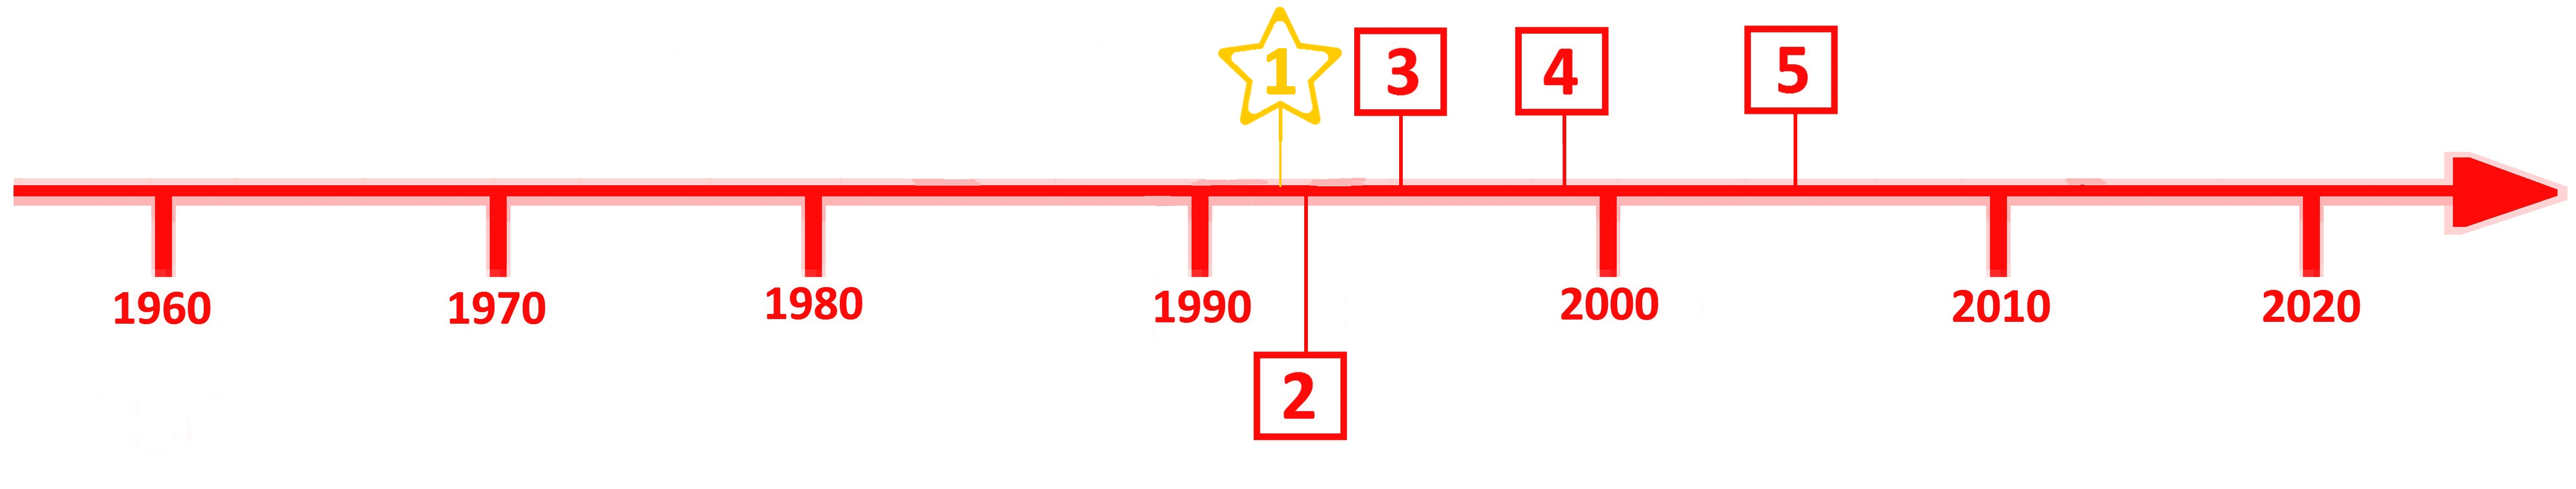
\includegraphics[width=\textwidth]{Kapitel/IrDA/Grafiken/Zeitstrahl.jpg}
\par
\noindent
\rowcolors{2}{}{\topicolor!20}
\begin{tabular}{p{0.5 cm}p{1.5 cm}p{15.55 cm}}
	Nr. & Datum & Entwicklungsschritte\\
	1 & 1993 & Die \textit{Infrared Data Association} wird gegründet.~\cite{wikipediade}\\
	2 & 1994 & IrDA 1.0 wird veröffentlicht. Der Standard entthält die Spezifikation von SIR, IrLAP und IrLMP.~\cite{irdahistory}\\
	3 & 1995 & IrPHY wird um MIR und FIR erweitert.~\cite{irdahistory}\\
	4 & 1999 & IrPHY wird um VFIR erweitert.~\cite{irdahistory}\\
	5 & 2005 & IrSimple wird spezifiziert.~\cite{wikipediade}\\
\end{tabular}
\par
\begin{multicols}{3}


\subsection*{Einsatz}
\begin{Figure}
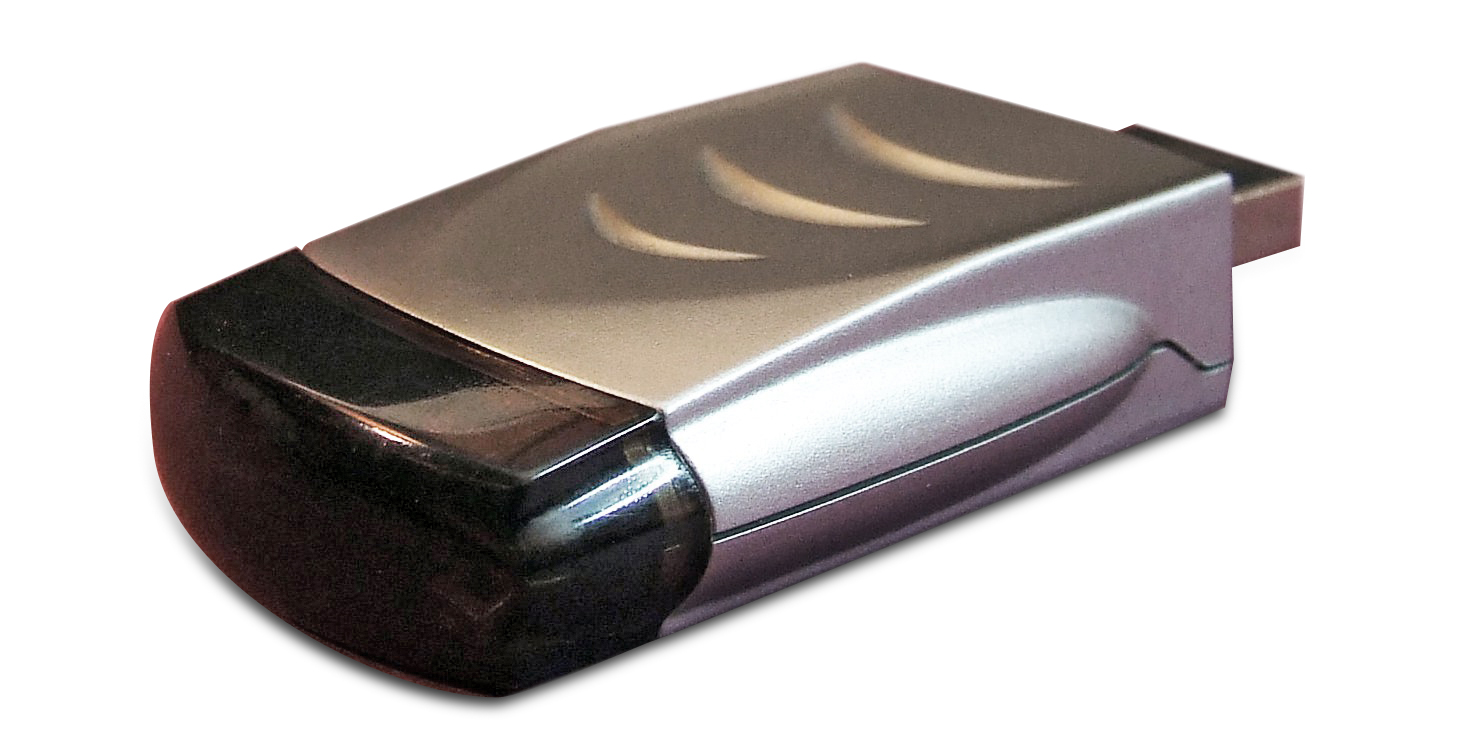
\includegraphics[width=\linewidth]{Kapitel/IrDA/Grafiken/irda_usb.jpg}
\captionof{figure}{Infrarot-USB-Modem für den PC~\cite{wikipediade}}
\label{fig:irda.modem}
\end{Figure}
Die IrDA-Protokollfamilie war rund um das Jahr 2000 weit verbreitet und wurde unter anderem auf PDAs, Notebooks und Handys im privaten und Enterprise-Umfeld eingesetzt.

Anfang der 2000er wurde IrDA und allgemein die Übertragung von Daten via IR mehr und mehr von Technologien auf Basis von Radiowellen, in erster Linie Bluetooth, verdrängt. Grund für diese Entwicklung war die Notwendigkeit, die Geräte für eine Übertragung via IR korrekt auszurichten. Bluetooth besitzt diese Einschränkung nicht und ist daher anwenderfreundlicher.

2005 gab es nochmals Versuche, IrDA mit den Weiterentwicklungen IrSimpleShot wiederzubeleben. IrSimple sollte dazu dienen, das Protokoll performanter zu gestalten, indem der Discovery-Prozess beschleunigt, sowie die Datenrate erhöht wurde. IrSimpleShot ist ein Protokoll auf Basis von IrSimple zur Übertragung von Fotos. Es sollte dazu dienen, Fotos von einer Kamera schnell zur genaueren Betrachtung auf ein Anzeigegerät zu übertragen. Ziel war die Übertragung innerhalb einer Sekunde.

Nach Meinung des Autors war IrSimple größtenteils erfolglos, IrDA-fähige Geräte sind immer noch ein Nischenprodukt. 

\subsection*{Anbieter und Gremien}
IrDA, das Gremium, welches die vorgestellten Protokolle definiert hat, hatte zu seiner Hochzeit circa 50 Mitgliedsunternehmen, darunter Microsoft, HP und IBM. Heute besitzt die IrDA nur noch ca. 25 Mitglieder und veröffentlicht sehr viel seltener neue Spezifikationen als früher.

Alle von der IrDA erstellten Dokumente stehen den Mitgliedern kostenlos zur Verfügung. Nichtmitglieder müssen die Spezifikationen kostenplichtig erwerben. Beispielsweise sind die sogenannten IrDA Core Specifications, also die Spezifikation der transportorientierten Protokolle wie IrPHY, IrLAP und IrLMP, zusammen für 670\$ erhältlich.

Eine Mitgliedschaft kostet zwischen 1500\$ und 8000\$ jährlich. Faktoren für die Kostenberechnung sind einerseits die Frage, ob das Mitglied Stimmrechte innerhalb der Organisation hat, und andererseits der jährliche Gewinn des Unternehmens.

\subsection*{Ausblick}
Die IrDA-Protokollfamilie wird wohl nicht mehr allzu lange weiterentwickelt werden. Zwar sind momentan noch Entwicklungen an 5/10GigaIR im Gange, jedoch dauern diese mittlerweile schon 5 Jahre an. Ob hier noch Ergebnisse zu erwarten sind, ist fraglich.

Microsoft hat mit Windows 10 auch den Support für den hauseigenen IrDA-Protokollstack eingestellt. Hierdurch können viele der Infrarot-Transceiver, die unter älteren Windows-Versionen noch funktionsfähig waren, nun nicht mehr genutzt werden. 

Durch diese und ähnliche Entwicklungen wird die Technologie wohl mittel- bis langfristig aussterben. Es erscheint höchst unwahrscheinlich, dass sich die Zahl der Nutzer nochmals erholt.

\printbibliography[segment=11,heading=subbibliography]
\end{multicols}

\newpage
